\chapter{Registro ARRT}


Il \textbf{registro ARRT}, ossia il progetto di partenza da cui sono stati ricavati i dati utilizzati per questa tesi, prende in considerazione pazienti di terapia intensiva sottoposti ad RRT.

Lo studio è stato svolto su molteplici centri ospedalieri, nello specifico 42 ed ha visto coinvolta una popolazione di circa 700 pazienti. Il registro tiene traccia dei primi dieci giorni di degenza nel reparto di terapia intensiva a partire dal momento di ingresso.

Analizzando i dati viene evidenziato come la tecnica del CRRT è stata quella più utilizzata, infatti viene  indicata su circa  l'87\% dei pazienti totali, questo è uno dei motivi per cui nei dati presi si sono considerati solamente i pazienti sottoposti a tale tecnica.
Anche nella scelta del filtro si è concentrato lo studio sui trattamenti con oXiris, applicato nel trattamento di circa 290 individui.

Ad oggi lo studio non è chiuso, pertanto i dati vengono ancora inseriti ed aggiornati. Al momento delle analisi, però, i pazienti studiati sono stati in numero minore, più o meno 270.

Per raccogliere i dati si è sfruttata la piattaforma REDCap, che è una web platform per costruire e gestire in modo sicuro database e sondaggi. Il processo semplificato di REDCap per la creazione e lo sviluppo rapido dei progetti, offre un vasto insieme di strumenti che può essere adattato praticamente a qualsiasi strategia di raccolta dati \cite{REDCap}. 


Per ogni soggetto sottoposto a terapia, i dati raccolti nel registro si dividono in: 
\begin{itemize}
	\itemsep -0.5 \parsep
	\item Anagrafica;
	\item Indicazione al Trattamento;
	\item Monitoraggi, che vanno dal giorno di ingresso in terapia intensiva fino al  decimo giorno di ricovero;
	\item Risultati finali.
\end{itemize}

Banalmente l'anagrafica contiene tutte le informazioni generiche del paziente (es sesso, età, razza ecc...) che ai fini dello studio non hanno un interesse specifico, infatti a tal proposito non si ritiene di interesse approfondirle.

\section{Indicazione al Trattamento}


Nell'indicazione al trattamento viene segnalato l'obiettivo di ricovero in terapia intensiva del paziente, che può essere:
\begin{enumerate}
	\itemsep -0.5 \parsep
	\item Supporto della funzione renale;
	\item Modulazione della risposta infiammatoria;
	\item Supporto della funzione renale e modulazione della risposta infiammatoria.
\end{enumerate}

\begin{figure}[h]
	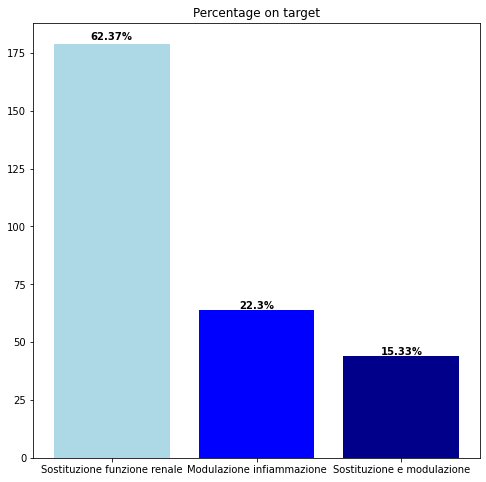
\includegraphics[width=8cm]{capitolo1/target.png}
	\centering
	\caption{Percentuale di distribuzione dei target rispetto i pazienti}
	\label{fig:target}
\end{figure}

Il supporto alla funzione renale è il trattamento più indicato tra gli obiettivi (figura \ref{fig:target}). In questa fase vengono, inoltre,  indicate 6 possibili cause o  indicazioni per cui è risultato necessario ricorrere alle terapie renali che sono le seguenti:
\begin{enumerate}
	\itemsep -0.5 \parsep
	\item   Fluid Overload;
	\item  Alterazione dei soluti;
	\item  Controllo dei soluti uremici;
	\item  Correzioni del bilancio acido/base;
	\item   Ipertermia;
	\item Drug overdose.
\end{enumerate}
Ovviamente queste vengono segnalate solamente per quei pazienti con problemi renali indicati nell'obiettivo.
Per ogni paziente può essere assegnata da una a più indicazioni alle terapie.
Un altro importante valore riportato nell'indicazioni al trattamento sono i lattati, che sono la forma ionizzata dell'acido lattico e sono utili per scoprire un'eventuale insufficienza renale.  
In questa fase vengono salvati solamente sui pazienti che riportano come obiettivo la modulazione della risposta infiammatoria (cioé sepsi), i lattati sono espressi con due unità di misura differenti che sono mmol/L oppure mg/dL, per omogeneizzare i dati si è deciso di considerarli tutti in unità mmol/L, convertendoli laddove necessario.

Le altre misurazioni presenti tra i valori delle indicazioni al trattamento non vengono presentate perché non utilizzate nelle analisi effettuate.

\section{Monitoraggi}

I monitoraggi vengono effettuati nei vari intervalli temporali che partono dal momento del ricovero, detto Tempo 0, fino al 10° giorno di degenza.
Le informazioni descritte, però, sono sempre le stesse pertanto è sufficiente descriverle una volta e, nello specifico, verranno prese in considerazioni alcune informazioni relative al tempo 0.

I parametri salvati possono essere suddivisi nelle seguenti categorie:
\begin{itemize}
	\itemsep -0.5 \parsep
	\item Cervello;
	\item Cuore;
	\item Polmoni;
	\item Reni;
	\item Fegato;
	\item Sepsi, Coronavirus e Score;
	\item Prescrizione al trattamento;
\end{itemize}

A seguire verranno esaminati in dettaglio.

\subsection{Cervello}

La \textbf{GCS} (Glasgow Coma Score) permette di fornire un primo grado di giudizio sulla gravità della sofferenza celebrale in corso. 
I parametri da cui si ricava il GCS sono 3 e sono:
\begin{itemize}
	\itemsep -0.5 \parsep
	\item \textbf{Apertura degli Occhi}, può avere un valore compreso tra 1 e 4, ogni rank rappresenta una risposta del paziente rispetto ad una certa condizione, nello specifico:
	
	\begin{center}
		\begin{tabular}{|c|c|}
		 \hline
		 \textbf{Risposta}&\textbf{Score}\\
		 \hline
		  Non Risposta & 1 \\
		  \hline
		  Risposta allo stimolo doloroso & 2 \\
		  \hline
		  Risposta allo stimolo verbale & 3 \\
		  \hline
		  Risposta spontanea & 4 \\
		  \hline		 
		\end{tabular}
	\end{center}

	\item \textbf{Risposta verbale}, il medico prende la propria decisione sul punteggio da assegnare basando le sue valutazioni sul rank a seguire:
	
		\begin{center}
		\begin{tabular}{|c|c|}
			\hline
			\textbf{Risposta}&\textbf{Score}\\
			\hline
			Non Risposta & 1 \\
			\hline
			Suoni incomprensibili & 2 \\
			\hline
			Parole inappropriate & 3 \\
			\hline
			Confusa & 4 \\
			\hline	
			Orientata & 5\\
			\hline		 
		\end{tabular}
	\end{center}

	Il valore può essere molto influenzato se il paziente necessita di un supporto per la respirazione che può fisicamente compromettere la risposta verbale.
	
	\item \textbf{Risposta motoria}, anche in questo caso si fa la valutazione in base allo stato attuale del paziente e si può definire un valore basandosi sulla classifica a seguire:
	
	\begin{center}
		\begin{tabular}{|c|c|}
			\hline
			\textbf{Risposta}&\textbf{Score}\\
			\hline
			Non Risposta & 1 \\
			\hline
			Estensione dell'arto al dolore & 2 \\
			\hline
			Flessione dell'arto al dolore & 3 \\
			\hline
			Allontanamento dell'arto al dolore & 4 \\
			\hline	
			Localizza il dolore & 5\\
			\hline	
			Esegue i comandi & 6\\
			\hline	 
		\end{tabular}
	\end{center}
\end{itemize}

La somma di questi valori permette di calcolare la GCS che al massimo può essere 15 e indica una condizione ottimale del paziente dal punto di vista del cervello, mentre il valore più basso è 3 che indica uno stato di coma totale del paziente.
Come si può vedere dalla tabella \ref{tab:gcs} è evidente come la maggior parte dei pazienti risultano in uno stato di incoscienza o semi incoscienza e sono molto pochi quelli abbastanza vigili.

\begin{table}[h!]
	\parbox{.45\textwidth}{
		\centering
		\begin{tabular}{ |p{3cm}|p{3cm} | }
			\hline
			\multicolumn{2}{|c|}{GCS} \\
			\hline \hline
			Score  & Numero pazienti  \\
			\hline \hline
			\textbf{3} & 195 \\
			\hline
			\textbf{4} & 5 \\
			\hline
			\textbf{5} & 8 \\
			\hline
			\textbf{6} & 11 \\
			\hline
			\textbf{7} & 8 \\
			\hline
			\textbf{8} & 5 \\
			\hline
		\end{tabular}}
	\quad
	\parbox{.45\textwidth}{
		\centering
		\begin{tabular}{ |p{3cm}|p{3cm} | }
			\hline 
			Score  & Numero pazienti  \\
			\hline \hline
			\textbf{9} & 4 \\
			\hline
			\textbf{10} & 5 \\
			\hline
			\textbf{11} & 4 \\
			\hline
			\textbf{12} & 2 \\
			\hline
			\textbf{13} & 13 \\
			\hline
			\textbf{14} & 8 \\
			\hline
			\textbf{15} & 27 \\
			\hline
		\end{tabular}}
	\caption{Tabella con il numero di pazienti rispetto al valore di Glasgow}
	\label{tab:gcs}
\end{table}

\subsection{Cuore}

Per quanto riguarda l'apparato cardiaco ci sono una serie di valori di interesse per determinare lo stato del paziente.
Tra i parametri più noti e più importanti risultano:
\begin{description}
	\itemsep -0.5 \parsep
		\item [Ritmo cardiaco]	può essere di tre tipologie: \textit{Ritmico, Aritmico, Pacemaker}, nei pazienti analizzati il ritmo più diffuso è quello ritmico (figura \ref{fig:ritmo}).
	\begin{figure}[h] 
		\centering
		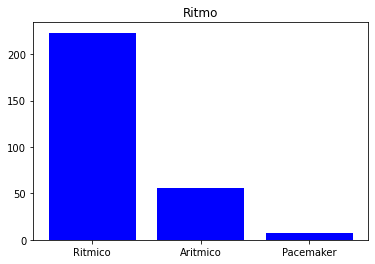
\includegraphics[width=0.30\textwidth]{capitolo1/ritmo.png}
		\caption{Valori del Ritmo nei pazienti nel registro}
		\label{fig:ritmo}
	\end{figure}
	\item[Arresto Cardiaco] indica se il paziente ha subito o meno un arresto cardiaco nelle ultime 24h e dai dati registrati il fenomeno si verifica solamente su 6 pazienti.
	\item[Frequenza Cadiaca](unità di misura bpm)  misura il numero di battiti al minuto e in media il valore è compreso tra i 60 e i 100 bpm. Nel registro i valori risultano compresi tra un minimo di 50 ad un massimo di 150 bpm.
	\item[Pressione Sistolica, Diastolica e Media] tutte e tre hanno come unità di misura mmHg. 
	La pressione sistolica (ps), o pressione massima,  è il valore della pressione arteriosa nel momento in cui il cuore è in fase di contrazione, al fine di spingere il sangue in circolo, in altre parole è la pressione sanguigna ad ogni battito del cuore, nei pazienti analizzati il valore varia tra 60 mmHg e 190mmHg. 
	La pressione diastolica (pd), o pressione minima, è il valore della pressione arteriosa nel momento in cui il cuore è in fase di rilassamento, in altre parole, è la pressione sanguigna tra due battiti cardiaci, nei pazienti il valore varia tra 30 mmHg e 95 mmHg.
	Da queste due pressioni si ricava la  pressione media la quale non è altro che una formula derivante dai precedenti due valori, infatti:
	$(ps * 0.333)+ (pd * 0.666)$, i valori variano nel registro tra 39.96 mmHg e 125.87 mmHg.
	\item [Temperatura] indica la temperatura corporea dei pazienti, si esprime in gradi Celsius e il  valore varia da 33°C a 41°C.
\end{description}

 Nella figura \ref{fig:cuore} sono mostrati i grafici delle distribuzioni per la frequenza, le pressioni e la temperatura.
\begin{figure}[h]
	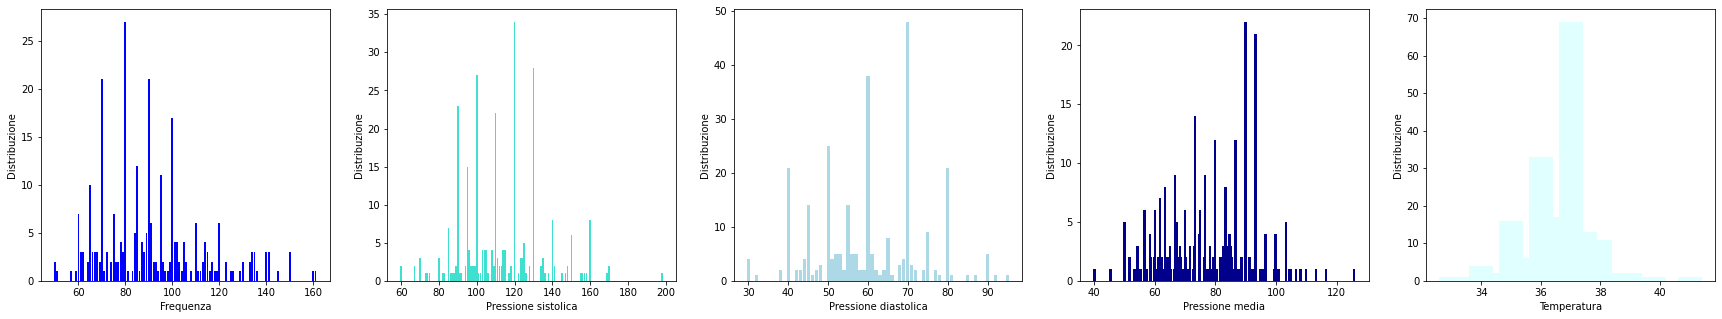
\includegraphics[width=15cm]{capitolo1/cuore.png}
	\centering
	\caption{Frequenza, pressione sistolica, pressione diastolica, pressione media e temperatura}
	\label{fig:cuore}
\end{figure}

Tra i valori più importanti analizzati associati al cuore si considerano farmaci vasoattivi. 
I farmaci vasoattivi sono sostanze in grado di agire sui centri nervosi deputati al controllo della motilità vasale (vasocostrizione e vasodilatazione). Sono indicati nello specifico 10 vaosattivi principali con i rispettivi dosaggi. Ad un paziente possono essere somministrati più vasoattivi. Al circa il 78\% della popolazione analizzata vengono somministrati vasoattivi.
I possibili vasoattivi somministrati sono: Adrenalina, Noradrenalina, Vasopressina, Idrocortisone, Dobutamina, Dopamina, Enoximone, Levosimendan, Terlipressina e Milrinone.
Le più usate risultano essere Adrenalina e Noradrenalina, mentre Enoximone e Milrinone non risultano mai utilizzate.
Combinando i dosaggi dei vasoattivi somministrati con altri parametri, come il peso, si può calcolare il \textbf{Vasoactive Inotropic Score} (VIS) che varia da un valore minimo di 0 ad un massimo di 200.

Andando avanti si trovano i monitoraggi cardiaci che possono essere di otto tipi: 
\begin{enumerate}
	\item Pressione Cruenta;
	\item Pressione non Invasiva;
	\item Ecocardiogramma;
	\item PRAM;
	\item Picco;
	\item Vigileo;
	\item EV1000;
	\item Swan - Ganz.
\end{enumerate}
I monitoraggi possono essere usati in maniera combinata, tra quelli più usati troviamo il monitoraggio con pressione cruenta e quello con ecocardiogramma, che vengono spesso combinati insieme. 
 
Gli altri dati cardiaci non vengono visti nel dettaglio perché risultano misurazioni non rilevanti allo scopo \\


\subsection{Polmoni}

Innanzitutto si procede a constatare quanti pazienti non hanno una respirazione spontanea, che risultano essere circa l'87\% del totale. Per questi ci sono 3 differenti interfacce di ventilazione:
\begin{itemize}
	\item Intubazione Oro-Tracheale;
	\item Tracheostomia;
	\item Ventilazione non invasiva.
\end{itemize}

Alle interfacce si accostano ulteriori 3 modalità di ventilazioni che sono le seguenti:

\begin{itemize}
	\item Controllata Pressumetrica;
	\item Controllata Volumetrica;
	\item Di supporto.
\end{itemize}

Nella figura \ref{fig:intermod} si può vedere su quanti pazienti sono applicate le differenti  interfacce e modalità di ventilazione, in particoolare dalla figura \ref{fig:inter} si può vedere come l'intubazione oro-tracheale sia l'interfaccia più usata, mentre sulle modalità, figura \ref{fig:moda} quella controllata volumetrica e quella di supporto risultano usate più o meno in uguale misura.
\begin{figure}[h]
	\begin{subfigure}{.5\textwidth}
		\centering
		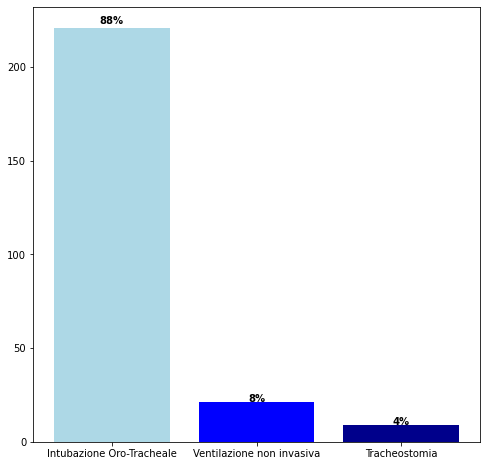
\includegraphics[width=.7\linewidth]{capitolo1/interfaccia.png}
		\caption{Interfacce}
		\label{fig:inter}
	\end{subfigure}%
	\begin{subfigure}{.5\textwidth}
		\centering
		\includegraphics[width=.7\linewidth]{capitolo1/modalità.png}
		\caption{Modalità di ventilazione}
		\label{fig:moda}
	\end{subfigure}
	\caption{Distribuzione dei pazienti rispetto alle interfacce e alle modalità di ventilazione}
	\label{fig:intermod}
\end{figure}

Nella tabella \ref{table:intermodalita} si può, inoltre, vedere su quanti pazienti vengono usate le interfacce in relazione a differenti modalità.

\begin{table}[h!]
	\centering
	\begin{tabular}{ |c| c|c|} 
		\hline
		\multicolumn{3}{|c|}{Respirazione assistita} \\
		\hline
		\textbf{Interfaccia} & \textbf{Modalità} & \textbf{Numero Pazienti} \\
		\hline
		\hline
		\multirow[t]{3}{*}{Intubazione Oro-Tracheale}& Controllata Pressumetrica & 96 \\  \cline{2-3}
		& Controllata Volumetrica & 100 \\  \cline{2-3}
		& Di supporto  & 23 \\  \cline{2-3}
		\hline
		\hline
		Tracheostomia & Di supporto & 9 \\
		\hline 
		\hline
		\multirow[t]{3}{*}{Ventilazione non invasiva} & 
		Controllata Pressumetrica & 5 \\  \cline{2-3}
		& Controllata Volumetrica & 11 \\  \cline{2-3}
		& Di supporto  & 5 \\  \cline{2-3}
		\hline 
	\end{tabular}
	\caption{Tabella di relazione tra interfacce e modalità.}
	\label{table:intermodalita}
\end{table}

Sui pazienti con respirazione assistita si valuta anche quello che è il volume polmonare, tra questi valori si considera il volume corrente o tidal, che rappresenta la quantità di aria che viene inspirata ed espirata ad ogni atto respiratorio. Nello specifico vengono salvate tre informazioni sul tidal:  desiderato, da importare ed impostato.
Il tidal desiderato rappresenta la quantità di aria desiderata che entra ed esce dai polmoni ad ogni atto respiratorio, il tidal da impostare rappresenta come bisogna impostare la macchina affinché si raggiungano effettivamente quelle quantità, mentre il tidal impostato rappresenta come viene effettivamente impostato il macchinario.
Dopo i dati volumetrici si passa ai dati pressori, che sono:il  peep, il picco pressorio, la pressione media delle vie aree e il plateu della pressione ed infine si trova la compliance polmonare, che unisce volume e pressione, infatti si definisce come la variazione del volume polmonare in seguito a variazioni unitarie della pressione applicate al polmone stesso, essa è dunque un indice della distensibilità della struttura.
Per quanto riguarda i pazienti con respirazione spontanea, invece, l'unico dato salvato è la quantità di flusso.

Tra i valori più rilevanti sui polmoni troviamo i lattati, che sono già stati descritti in precedenza, ma in questo caso vengono registrati per ogni paziente, anche ora come unica unità di misura si considera il mmol/L.
L'ultimo dato considerato in relazione ai polmoni è l'ematocrito (hct), è registrato come un valore percentuale, che in media è intorno al 30\%.
Nella figura \ref{fig:hct} si può vedere come si ditribuisce l'hct e ancora più nel dettaglio nella figura \ref{fig:hct1} viene mostrato l'hct per i pazienti senza respirazione spontanea (in azzurro) e per quelli che respirano spontaneamente (in blu).


\begin{figure}[h]
	\begin{subfigure}{.5\textwidth}
		\centering
		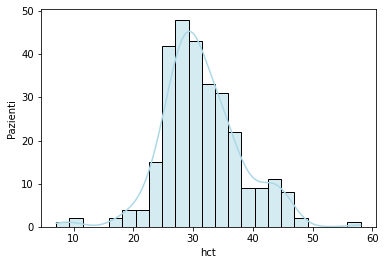
\includegraphics[width=.8\linewidth]{capitolo1/hct.png}
		\caption{Hct su tutti i pazienti}
		\label{fig:hct}
	\end{subfigure}%
	\begin{subfigure}{.5\textwidth}
		\centering
		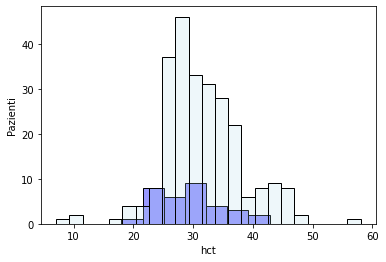
\includegraphics[width=.8\linewidth]{capitolo1/hct1.png}
		\caption{hct diviso per i tipi di pazienti}
		\label{fig:hct1}
	\end{subfigure}
\end{figure}



\subsection{Reni}

Importantissimo per determinare se ci possa essere un danno renale è il valore della creatinina.
Se il rene funziona la cretinina ha un valore  intorno a 1 mg/dL.
I valori in media però sono leggermente più alti, infatti ho un valore medio di 3,12 mg/dL (figura \ref{fig:crea}).

\begin{figure}[h] 
	\centering
	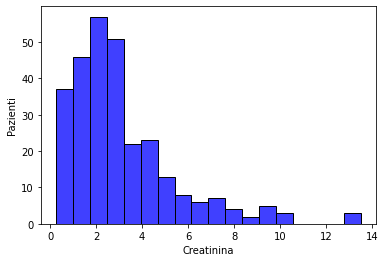
\includegraphics[width=10cm]{capitolo1/crea.png}
	\caption{Valori della Creatinina nei pazienti nel registro}
	\label{fig:crea}
\end{figure}

Anche l'output urinario rappresenta un importante fattore per determinare il funzionamento del rene, su alcuni pazienti l'output urinario è pari a zero e sono tutti quei pazienti che necessitano di supporto nella terapia renale e con un fluidoverload registrato nella fase di indicazione al trattamento, in genere infatti per questi pazienti è indicata una terapia diuretica. Il valore medio dell'output urinario è di circa 69 ml/h.
 
\subsection{Fegato}
Sui valori del fegato interessanti ci sono certamente: bilirubina, albumina e piastrine.
Per quanto riguarda l'albumina il valore normale è di 0.8 mg/dl, anche se il livello medio risulta di 2,58 mg/dl.
Le albumine e le piastrine hanno una media di 3,9 g/dl e 191 $10^3$/microlitro, la loro distribuzione è visibile rispettivamente nelle figure \ref{fig:alb} e \ref{fig:piastr}.

\begin{figure}[h]
	\begin{subfigure}{.5\textwidth}
		\centering
		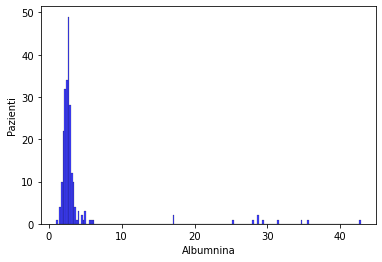
\includegraphics[width=.8\linewidth]{capitolo1/alb.png}
		\caption{Albuminei}
		\label{fig:alb}
	\end{subfigure}%
	\begin{subfigure}{.5\textwidth}
		\centering
		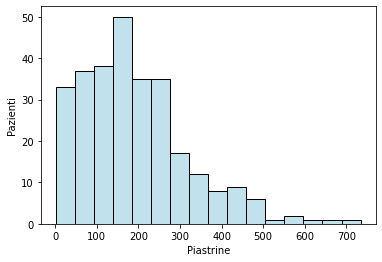
\includegraphics[width=.8\linewidth]{capitolo1/piastrine.png}
		\caption{Piastrine}
		\label{fig:piastr}
	\end{subfigure}
\end{figure}

Vengono tralasciati ulteriori valori misurati del fegato, perché in generale risultano avere un impatto secondario.

\subsection{Sepsi, Coronavirus e Score}

La sepsi è una sindrome clinica di disfunzioni organiche potenzialmente letale causata da una risposta disregolata all'infezione. Nello shock settico si verifica una riduzione critica della perfusione dei tessuti che può condurre a uno stato di insufficienza multiorgano che coinvolge polmoni, reni e fegato. Nella popolazione studiata si può vedere come il numero di pazienti septici è una percentuale consistente (figura \ref{fig:sepsi}), in parte era prevedibile considerando gli obiettivi di ricovero nelle indicazioni al trattamento.

\begin{figure}[h] 
	\centering
	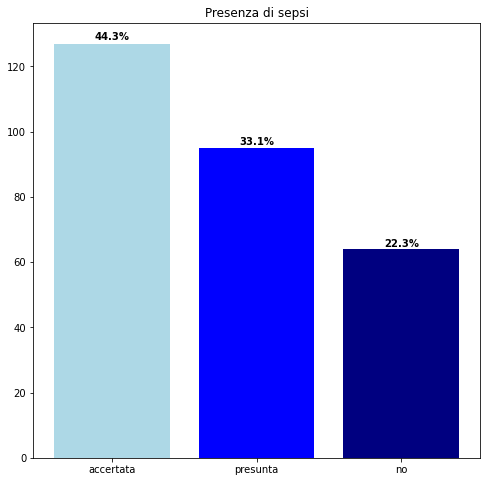
\includegraphics[width=8cm]{capitolo1/sepsi.png}
	\caption{Percentuale della sepsi, che può essere accertata, presunta o proprio non considerata }
	\label{fig:sepsi}
\end{figure}

Ci sono sette differenti sedi in cui la sepsi può essere riscontrata che possono essere più di una contemporaneamente. Le sedi sono:
\begin{itemize}
	\item Apparato respiratorio;
	\item Endoaddominale;
	\item Apparato urinario;
	\item Tessuti molli;
	\item Sistema nervoso centrale;
	\item Batteriemia.
\end{itemize}

Importante è anche l'indagine effettuata sul covid, in generale non viene sempre indagata, ma potrebbe rappresentare interessante vedere anche come si relaziona con la sepsi. In figura  \ref{fig:covid} si può vedere come si distribuisce il coronavirus rispetto i pazienti. 
\begin{figure}[h] 
	\centering
	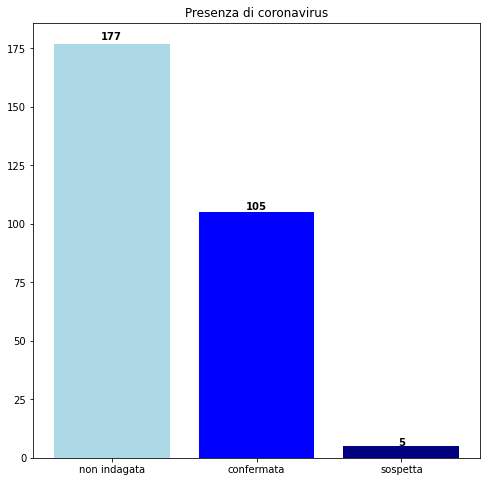
\includegraphics[width=6cm]{capitolo1/covid.png}
	\caption{Distribuzione del coronavirus sui pazienti}
	\label{fig:covid}
\end{figure}

Nella tabella \ref{table:sepcov} si può vedere come si distribuiscono i pazienti rispetto a sepsi e coronavirus.
\begin{table}[h]
	\centering
	\begin{tabular}{  |c| c|c|} 
		\hline
		\textbf{Sepsi} & \textbf{Coronavirus} & \textbf{Pazienti}  \\
		\hline
		\multirow[t]{3}{*}{No} & Sospetta & 1 \\  \cline{2-3}
		& Confermata & 48 \\  \cline{2-3}
		& Non indagata & 15 \\
		\hline                            
		\multirow[t]{3}{*}{Presunta} & Sospetta & 2  \\ \cline{2-3}
		& Confermata & 16 \\ \cline{2-3}
		& Non indagata & 77 \\ 
		\hline
		\multirow[t]{3}{*}{Accertata} & Sospetta & 2 \\ \cline{2-3}
		& Confermata & 41 \\ \cline{2-3}
		& Non indagata & 84 \\  
		\hline 
	\end{tabular}
	\caption{Distribuzione dei pazienti con coronavirus raggruppati per sepsi.}
	\label{table:sepcov}
\end{table}



Un altro importante valore che può avere un impatto sulla sepsi sono i valori dei globuli bianchi. 
I globuli bianchi, chiamati anche leucociti, sono cellule presenti nel sangue che fanno parte del sistema immunitario a cui è demandato il compito di difendere l’organismo dall’attacco portato da microrganismi patogeni o da corpi estranei che penetrano nell’organismo attraverso la cute o le mucose.
In generale i valori intorno a 1000 millilitri e sui 30000  millilitri determinano che il paziente non è in buono stato, mentre i pazienti con i valori di globuli bianchi compresi tra 5000  millilitri  e 10000 millilitri dovrebbero indicare uno stato normale, questo però non è sempre vero, infatti nel caso in cui questi pazienti risultano avere uno stato di sepsi confermata, non si possono considerare in uno stato di benessere.
Questo permette di suddividere i pazienti in due gruppi, il primo che comprende tutti quei pazienti a cui l'organismo reagisce con una risposta infiammatoria esagerata, portando perciò i valori di globuli bianchi a livelli estremi e il secondo gruppo che comprende tutti quei pazienti \textit{anergici} con sepsi, ossia coloro che non riescono a montare una risposta all'infiammazione.

Nello studio effettuato si considerano tre differenti modi per calcolare lo score di mortalità e sono: 
\begin{description}
	\itemsep -0.5 \parsep
	\item[APACHI Score] è un acronimo che significa \textit{Acute Physiologic Assessment and Chronic Health Evaluation}, è il punteggio finale ottenuto da una serie di punteggi assegnati a determinati parametri vitali, esami ematochimici e notizie di natura amnestica (es temperatura, pressione, ossigenazione, GCS, ecc...).
	A seconda del punteggio si ricava una percentuale di mortalità, più lo score è basso più è bassa la percentuale ;
	\item[SOFA Score] acronimo di \textit{Sequential Organ Failure Assessment}, è un punteggio clinico utilizzato per valutare lo stato del paziente durante il ricovero nella terapia intensiva. Esso determina l’estensione delle funzioni o dei danni degli organi del paziente.
	Il SOFA è calcolato come somma dei punteggi derivanti dall'analisi di 6 sistemi (respiratorio, cardiovascolare, epatico, coagulatorio, renale, neurologico) graduati da 0 a 4 in accordo col grado di disfunzione o danno del sistema considerato. Anche in questo caso un punteggio alto totale indica un stato peggiore del paziente
	\item[SAP Score] acronimo di \textit{Simplified Acute Physiology} 	questo sistema è particolarmente usato per descrivere la morbidità del paziente confrontata con i risultati di un’altro paziente e per descrivere la morbidità di un gruppo di pazienti confrontata con i risultati di un’altro gruppo di pazienti.
	Il punteggio finale (intero compreso tra 0 e 163) è calcolato attraverso la somma dei punteggi parziali associati a 15 misure fisiologiche usuali di cui dev'essere scelto il peggior valore registrato durante le prime 24 ore di ricovero in terapia intensiva.
	L'applicativo calcola, inoltre, la probabilità (\%) di morte del paziente.
\end{description}


\subsection{Prescrizione al trattamento}

In questa sezione si trovano tutti i valori fondamentali di riferimento per l'RRT, per esempio qui si dichiara il tipo di terapia e di filtro usati. Ci sono molteplici valori significativi tra quelli memorizzati nella prescrizione al trattamento, ma per semplicità se ne descrive uno ossia gli anticoagulanti.
\begin{figure}[h] 
	\centering
	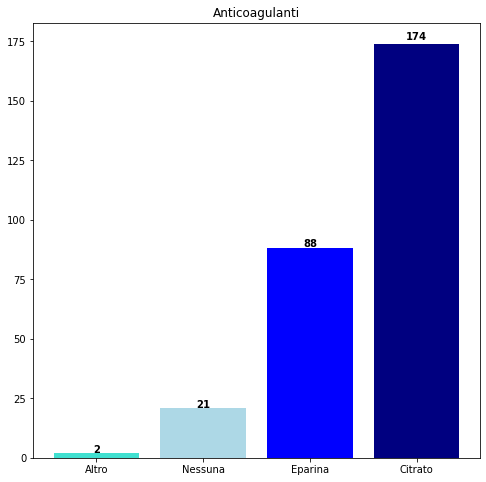
\includegraphics[width=6cm]{capitolo1/anticoag.png}
	\caption{Anticoagulanti utilizzati nello studio}
	\label{fig:antico}
\end{figure}\\
Nello specifico i farmaci anticoagulanti sono farmaci capaci di ostacolare la coagulazione del sangue. Vista la loro azione terapeutica, questi farmaci vengono utilizzati per prevenire la formazione di trombi e per ostacolare l'accrescimento di quelli che si sono già formati. Come si puo vedere nella figura \ref{fig:antico} quello più utilizzato risulta essere il citrato, seguito dall'eparina.





\section{Risultati finali}

In questa ultima sezione vengono registrati tutti i dati alla fine dei trattamenti, che  possono concludersi per decesso del paziente o per dimissione (figura \ref{fig:dece}).

\begin{figure}[h] 
	\centering
	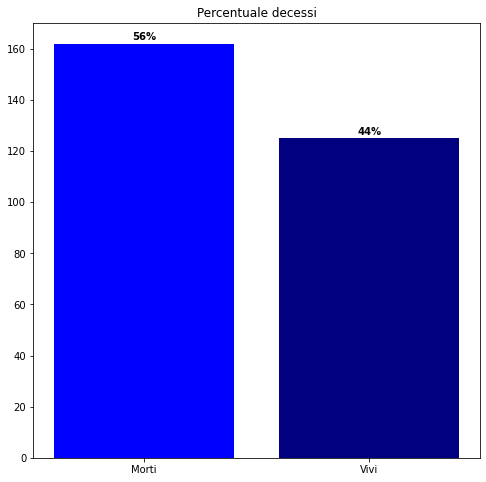
\includegraphics[width=6cm]{capitolo1/decessi.png}
	\caption{Percentuale degli esiti di terapia intensiva}
	\label{fig:dece}
\end{figure}

Analizzando i giorni di ricovero si ha che la media si aggira intorno ai 13 giorni,  considerando, però, i pazienti in maniera separata  si ha una media di 10 giorni per i pazienti deceduti, mentre una di 18 giorni per i pazienti che sopravvivono.
Anche tra i risultati finali si trovano molteplici valori, ma non è lo scopo finale di questo lavoro analizzarli nel dettaglio.

